\documentclass{standalone}
\usepackage{tikz}
\usetikzlibrary{patterns, positioning}

\begin{document}
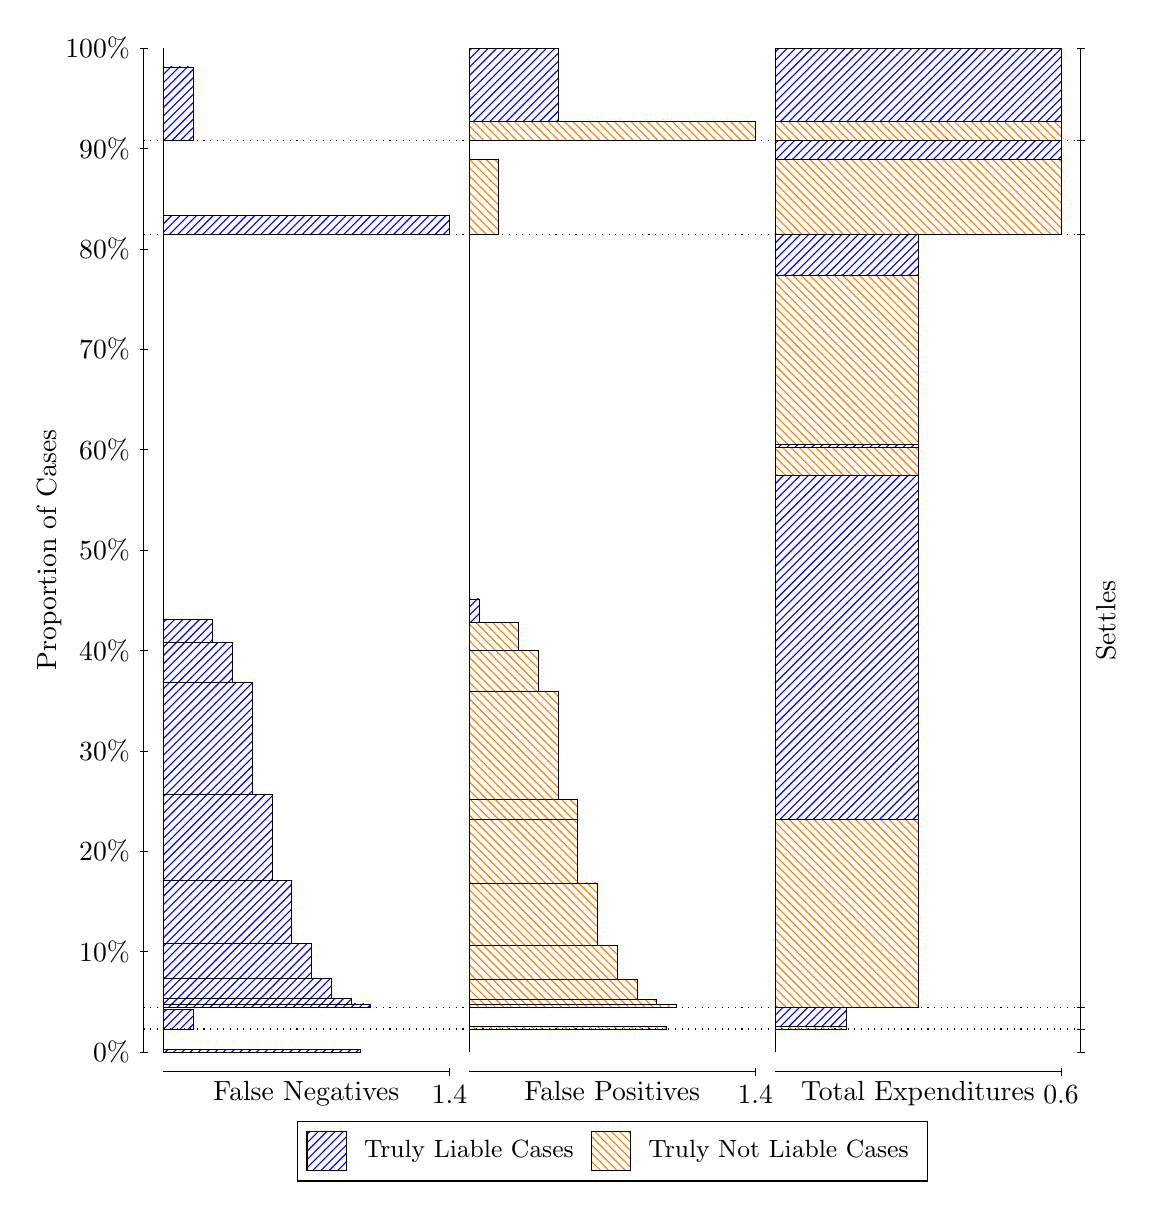
\begin{tikzpicture}
\draw[black, very thin] (1.5,1.75) -- (1.5,14.5);
\node[rotate=90, anchor=center] at (0.3, 8.125) {Proportion of Cases};
\draw[black, very thin] (1.45,1.75) -- (1.55,1.75);
\node[anchor=east] at (1.45, 1.75) {0\%};
\draw[black, very thin] (1.45,3.025) -- (1.55,3.025);
\node[anchor=east] at (1.45, 3.025) {10\%};
\draw[black, very thin] (1.45,4.3) -- (1.55,4.3);
\node[anchor=east] at (1.45, 4.3) {20\%};
\draw[black, very thin] (1.45,5.575) -- (1.55,5.575);
\node[anchor=east] at (1.45, 5.575) {30\%};
\draw[black, very thin] (1.45,6.85) -- (1.55,6.85);
\node[anchor=east] at (1.45, 6.85) {40\%};
\draw[black, very thin] (1.45,8.125) -- (1.55,8.125);
\node[anchor=east] at (1.45, 8.125) {50\%};
\draw[black, very thin] (1.45,9.4) -- (1.55,9.4);
\node[anchor=east] at (1.45, 9.4) {60\%};
\draw[black, very thin] (1.45,10.675) -- (1.55,10.675);
\node[anchor=east] at (1.45, 10.675) {70\%};
\draw[black, very thin] (1.45,11.95) -- (1.55,11.95);
\node[anchor=east] at (1.45, 11.95) {80\%};
\draw[black, very thin] (1.45,13.225) -- (1.55,13.225);
\node[anchor=east] at (1.45, 13.225) {90\%};
\draw[black, very thin] (1.45,14.5) -- (1.55,14.5);
\node[anchor=east] at (1.45, 14.5) {100\%};

\draw[black, very thin] (13.4,1.75) -- (13.4,14.5);
\draw[black, very thin] (13.35,1.75) -- (13.45,1.75);
\node[anchor=west] at (13.35, 1.75) {};
\draw[black, very thin] (13.35,2.042) -- (13.45,2.042);
\node[anchor=west] at (13.35, 2.042) {};
\draw[black, very thin] (13.35,2.3186) -- (13.45,2.3186);
\node[anchor=west] at (13.35, 2.3186) {};
\draw[black, very thin] (13.35,12.134) -- (13.45,12.134);
\node[anchor=west] at (13.35, 12.134) {};
\draw[black, very thin] (13.35,13.331) -- (13.45,13.331);
\node[anchor=west] at (13.35, 13.331) {};
\draw[black, very thin] (13.35,14.5) -- (13.45,14.5);
\node[anchor=west] at (13.35, 14.5) {};

\draw[black, very thin, pattern color=blue, pattern=north east lines] (1.75,1.75) rectangle (4.2557,1.7807);
\draw[black, very thin, pattern color=orange, pattern=north west lines] (1.75,1.7807) rectangle (1.75,2.042);
\draw[black, very thin, pattern color=blue, pattern=north east lines] (1.75,2.042) rectangle (2.1259,2.2896);
\draw[black, very thin, pattern color=orange, pattern=north west lines] (1.75,2.2896) rectangle (1.75,2.3186);
\draw[black, very thin, pattern color=blue, pattern=north east lines] (1.75,2.3186) rectangle (4.381,2.3621);
\draw[black, very thin, pattern color=blue, pattern=north east lines] (1.75,2.3621) rectangle (4.1305,2.4306);
\draw[black, very thin, pattern color=blue, pattern=north east lines] (1.75,2.4306) rectangle (3.8799,2.6816);
\draw[black, very thin, pattern color=blue, pattern=north east lines] (1.75,2.6816) rectangle (3.6293,3.1256);
\draw[black, very thin, pattern color=blue, pattern=north east lines] (1.75,3.1256) rectangle (3.3787,3.9327);
\draw[black, very thin, pattern color=blue, pattern=north east lines] (1.75,3.9327) rectangle (3.1282,5.0218);
\draw[black, very thin, pattern color=blue, pattern=north east lines] (1.75,5.0218) rectangle (2.8776,6.4458);
\draw[black, very thin, pattern color=blue, pattern=north east lines] (1.75,6.4458) rectangle (2.627,6.9471);
\draw[black, very thin, pattern color=blue, pattern=north east lines] (1.75,6.9471) rectangle (2.3764,7.246);
\draw[black, very thin, pattern color=orange, pattern=north west lines] (1.75,7.246) rectangle (1.75,12.134);
\draw[black, very thin, pattern color=blue, pattern=north east lines] (1.75,12.134) rectangle (5.3833,12.374);
\draw[black, very thin, pattern color=orange, pattern=north west lines] (1.75,12.374) rectangle (1.75,13.331);
\draw[black, very thin, pattern color=blue, pattern=north east lines] (1.75,13.331) rectangle (2.1259,14.26);
\draw[black, very thin, pattern color=orange, pattern=north west lines] (1.75,14.26) rectangle (1.75,14.5);
\draw[black, very thin, pattern color=orange, pattern=north west lines] (5.6333,1.75) rectangle (5.6333,2.0113);
\draw[black, very thin, pattern color=blue, pattern=north east lines] (5.6333,2.0113) rectangle (5.6333,2.042);
\draw[black, very thin, pattern color=orange, pattern=north west lines] (5.6333,2.042) rectangle (8.1391,2.071);
\draw[black, very thin, pattern color=blue, pattern=north east lines] (5.6333,2.071) rectangle (5.6333,2.3186);
\draw[black, very thin, pattern color=orange, pattern=north west lines] (5.6333,2.3186) rectangle (8.2644,2.3562);
\draw[black, very thin, pattern color=orange, pattern=north west lines] (5.6333,2.3562) rectangle (8.0138,2.4219);
\draw[black, very thin, pattern color=orange, pattern=north west lines] (5.6333,2.4219) rectangle (7.7632,2.6713);
\draw[black, very thin, pattern color=orange, pattern=north west lines] (5.6333,2.6713) rectangle (7.5126,3.1081);
\draw[black, very thin, pattern color=orange, pattern=north west lines] (5.6333,3.1081) rectangle (7.2621,3.8962);
\draw[black, very thin, pattern color=orange, pattern=north west lines] (5.6333,3.8962) rectangle (7.0115,4.7059);
\draw[black, very thin, pattern color=orange, pattern=north west lines] (5.6333,4.7059) rectangle (7.0115,4.9547);
\draw[black, very thin, pattern color=orange, pattern=north west lines] (5.6333,4.9547) rectangle (6.7609,6.3334);
\draw[black, very thin, pattern color=orange, pattern=north west lines] (5.6333,6.3334) rectangle (6.5103,6.8546);
\draw[black, very thin, pattern color=orange, pattern=north west lines] (5.6333,6.8546) rectangle (6.2598,7.2064);
\draw[black, very thin, pattern color=blue, pattern=north east lines] (5.6333,7.2064) rectangle (5.7586,7.5053);
\draw[black, very thin, pattern color=blue, pattern=north east lines] (5.6333,7.5053) rectangle (5.6333,12.134);
\draw[black, very thin, pattern color=orange, pattern=north west lines] (5.6333,12.134) rectangle (6.0092,13.09);
\draw[black, very thin, pattern color=blue, pattern=north east lines] (5.6333,13.09) rectangle (5.6333,13.331);
\draw[black, very thin, pattern color=orange, pattern=north west lines] (5.6333,13.331) rectangle (9.2667,13.571);
\draw[black, very thin, pattern color=blue, pattern=north east lines] (5.6333,13.571) rectangle (6.7609,14.5);
\draw[black, very thin, pattern color=orange, pattern=north west lines] (9.5167,1.75) rectangle (9.5167,2.0113);
\draw[black, very thin, pattern color=blue, pattern=north east lines] (9.5167,2.0113) rectangle (9.5167,2.042);
\draw[black, very thin, pattern color=orange, pattern=north west lines] (9.5167,2.042) rectangle (10.425,2.071);
\draw[black, very thin, pattern color=blue, pattern=north east lines] (9.5167,2.071) rectangle (10.425,2.3186);
\draw[black, very thin, pattern color=orange, pattern=north west lines] (9.5167,2.3186) rectangle (11.333,4.7059);
\draw[black, very thin, pattern color=blue, pattern=north east lines] (9.5167,4.7059) rectangle (11.333,9.0743);
\draw[black, very thin, pattern color=orange, pattern=north west lines] (9.5167,9.0743) rectangle (11.333,9.4261);
\draw[black, very thin, pattern color=blue, pattern=north east lines] (9.5167,9.4261) rectangle (11.333,9.4697);
\draw[black, very thin, pattern color=orange, pattern=north west lines] (9.5167,9.4697) rectangle (11.333,11.618);
\draw[black, very thin, pattern color=blue, pattern=north east lines] (9.5167,11.618) rectangle (11.333,12.134);
\draw[black, very thin, pattern color=orange, pattern=north west lines] (9.5167,12.134) rectangle (13.15,13.09);
\draw[black, very thin, pattern color=blue, pattern=north east lines] (9.5167,13.09) rectangle (13.15,13.331);
\draw[black, very thin, pattern color=orange, pattern=north west lines] (9.5167,13.331) rectangle (13.15,13.571);
\draw[black, very thin, pattern color=blue, pattern=north east lines] (9.5167,13.571) rectangle (13.15,14.5);
\draw[black, dotted] (1.5,2.042) -- (13.4,2.042);
\draw[black, dotted] (1.5,2.3186) -- (13.4,2.3186);
\draw[black, dotted] (1.5,12.134) -- (13.4,12.134);
\draw[black, dotted] (1.5,13.331) -- (13.4,13.331);
\draw[black, very thin] (1.75,1.5) -- (5.3833,1.5);
\node[anchor=north] at (3.5667, 1.5) {False Negatives};
\draw[black, very thin] (5.3833,1.45) -- (5.3833,1.55);
\node[anchor=north] at (5.3833, 1.45) {1.4};

\draw[black, very thin] (5.6333,1.5) -- (9.2667,1.5);
\node[anchor=north] at (7.45, 1.5) {False Positives};
\draw[black, very thin] (9.2667,1.45) -- (9.2667,1.55);
\node[anchor=north] at (9.2667, 1.45) {1.4};

\draw[black, very thin] (9.5167,1.5) -- (13.15,1.5);
\node[anchor=north] at (11.333, 1.5) {Total Expenditures};
\draw[black, very thin] (13.15,1.45) -- (13.15,1.55);
\node[anchor=north] at (13.15, 1.45) {0.6};



\node[black, centered, rotate=90] at (13.72, 7.2262) {Settles};



\draw (7.449999999999999,1.5) node[draw=none] (baseCoordinate) {};
\begin{scope}[align=center]
        \matrix[scale=0.5, draw=black, below=0.5cm of baseCoordinate, nodes={draw}, column sep=0.1cm]{
            \node[rectangle, draw, minimum width=0.5cm, minimum height=0.5cm, pattern=north east lines, pattern color=blue] {}; &
            \node[draw=none, font=\small] (B) {Truly Liable Cases}; &
            \node[rectangle, draw, minimum width=0.5cm, minimum height=0.5cm, pattern=north west lines, pattern color=orange] {}; &
            \node[draw=none, font=\small] (B) {Truly Not Liable Cases}; \\
            };
\end{scope}

\end{tikzpicture}
\end{document}